%++++++++++++++++++++++++++++++++++++++++
% Don't modify this section unless you know what you're doing!
\documentclass[letterpaper,12pt]{article}
\usepackage{tabularx} % extra features for tabular environment
\usepackage{amsmath}  % improve math presentation
\usepackage{graphicx} % takes care of graphic including machinery
\usepackage[margin=1in,letterpaper]{geometry} % decreases margins
\usepackage{cite} % takes care of citations
\usepackage[final]{hyperref} % adds hyper links inside the generated pdf file
\usepackage{pgfplotstable, booktabs}
\usepackage{placeins}
\usepackage{tabularray}
\usepackage{titlesec}
\usepackage{fancyhdr}
\usepackage{empheq}
\usepackage{amssymb}
\usepackage{sectsty}
\usepackage{tcolorbox}
\usepackage{listings}
\usepackage{xcolor}
\usepackage{parskip}
\usepackage{siunitx}
\usepackage{cancel}
\usepackage{enumitem}
\usepackage{subcaption}
\usepackage{caption}

\definecolor{codegreen}{rgb}{0,0.6,0}
\definecolor{codegray}{rgb}{0.5,0.5,0.5}
\definecolor{codepurple}{rgb}{0.58,0,0.82}

\lstdefinestyle{mystyle}{
    commentstyle=\color{codegreen},
    keywordstyle=\color{codepurple},
    numberstyle=\tiny\color{codegray},
    stringstyle=\color{codegreen},
    basicstyle=\ttfamily\small,
    breakatwhitespace=false,         
    breaklines=true,                 
    captionpos=b,                    
    keepspaces=true,                                                     
    showspaces=false,                
    showstringspaces=false,
    showtabs=false,                  
    tabsize=4
}

\lstset{style=mystyle}
  
\newcommand*\widefbox[1]{\fbox{\hspace{0em}#1\hspace{0em}}}

% new command for trace = tr()
\newcommand{\tr}{\text{tr}}

\pagestyle{fancy}
\fancyhf{} % Clear all header and footer fields
\fancyhead[L]{MEC E 380}
%\fancyhead[C]{Center Header}
\fancyhead[C]{Assignment 4}
\fancyhead[R]{Alex Diep}

\fancyfoot[C]{\thepage}

\pgfplotsset{compat=1.18} 
\titleformat*{\section}{\Large\bfseries}
\titleformat*{\subsection}{\large\bfseries}

\renewcommand{\thesection}{Question \arabic{section}}
\renewcommand{\thesubsection}{(\alph{subsection})}

% remove siunitx grouping
\sisetup{group-separator={}}

\hypersetup{
	colorlinks=true,       % false: boxed links; true: colored links
	linkcolor=blue,        % color of internal links
	citecolor=blue,        % color of links to bibliography
	filecolor=magenta,     % color of file links
	urlcolor=blue         
}
%++++++++++++++++++++++++++++++++++++++++
\begin{document}
% \begin{titlepage}
%     \centering
%     \vspace*{2cm} % Adjust vertical spacing
    
%     % Title
%     \Huge {MEC E 301 \\Lab 1: Dimensional Measurement} \\
%     \vspace{1cm} % Adjust vertical spacing
    
%     % Author
%     \Large by: Alex Diep \\
%     \vspace{1cm} % Adjust vertical spacing

%     % Date
%     \Large Date: September 19, 2023 \\ % or manually specify a date
%     \vspace{4cm} % Adjust vertical spacing

%     % CCID and Student ID in smtaller font
%     \normalsize CCID: abdiep \\
%     \normalsize Student ID: 1664334 \\ 
%     \normalsize Section: D21 \\
    
%     \vfill % Fill vertical space
    
%     % Additional content (e.g., university logo or other information)
    
% \end{titlepage}
\renewcommand\arraystretch{1.5}

\section{}
At a point in a loaded body, the stress relative to an x, y, and z coordinate system are 

\begin{equation}
    \sigma = 
    \begin{bmatrix}
        40 & 40 & 30 \\
        40 & 20 & 0 \\
        30 & 0 & 20
    \end{bmatrix}
    %units are mpa
    \unit{MPa} \nonumber
\end{equation} 

Determine the normal stress $\sigma$ and the shearing stress $\tau$ on a plane whose outward normal is
oriented at angles of 40$^\circ$, 75$^\circ$, and 54$^\circ$ with the x, y, and z axes, respectively.

First calculate the normal vector:
\begin{align}
    \hat{n} &= 
    \begin{bmatrix}
        \cos(40^\circ) \\
        \cos(75^\circ) \\
        \cos(54^\circ)
    \end{bmatrix} \nonumber 
\end{align}

Then calculate the normal stress:
\begin{align}
    \sigma_n &= \hat{n}^T \sigma \hat{n} \nonumber \\
    &= 
    \begin{bmatrix}
        \cos(40^\circ) & \cos(75^\circ) & \cos(54^\circ)
    \end{bmatrix}
    \begin{bmatrix}
        40 & 40 & 30 \\
        40 & 20 & 0 \\
        30 & 0 & 20
    \end{bmatrix}
    \begin{bmatrix}
        \cos(40^\circ) \\
        \cos(75^\circ) \\
        \cos(54^\circ)
    \end{bmatrix} \nonumber \\
    &= \boxed{\qty{74.6}{MPa}} \nonumber
\end{align}

To determine shearing stress magnitude, the following equation is used:
\begin{align}
    \tau &= \sqrt{p_{x}^2 + p_{y}^2 + p_{z}^2 - \sigma_n^2} \nonumber \\
    & = ((\sigma\hat{n})^T (\sigma\hat{n}) - \sigma_n^2)^{1/2} \nonumber \\
    & = (5926.856 - 5565.16)^{1/2} \nonumber \\
    &= \boxed{\qty{19.02}{MPa}} \nonumber
\end{align}
% \section{}
Referring to Figure \ref{fig:Q2ProblemDiagram}, verify the results 
\begin{align*}
    \int_{0}^{\pi/2} (\sigma_r \sin\theta) r d\theta = \int_{0}^{\pi/2} \frac{2P}{\pi} \sin\theta \cos\theta d\theta = \frac{P}{\pi} \\
    \int_{-\pi/2}^{\pi/2} (\sigma_\theta \cos\theta) r d\theta = \int_{-\pi/2}^{\pi/2}\frac{2P}{\pi} \cos^2\theta d\theta = P 
\end{align*}
\begin{figure}[h]
    \centering
    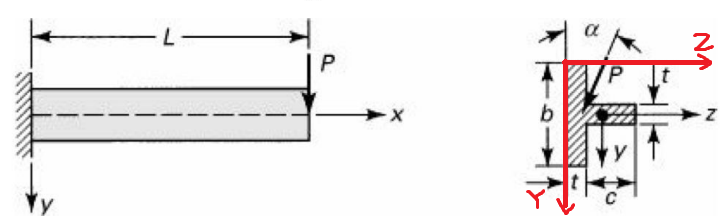
\includegraphics[width=0.35\linewidth]{Questions/Figures/Q2ProblemDiagram.png}
    \caption{Problem diagram for Question 2.}
    \label{fig:Q2ProblemDiagram}
\end{figure}

For radial stress distribution in a very large plate (semi-infinite solid) under normal load at its horizontal surface,
(Eq. 3.48 in the textbook)
\begin{equation*}
    \sigma_r = \frac{2P}{\pi r} \cos\theta
\end{equation*}
Verifying the first integral,
\begin{align*}
    \int_{0}^{\pi/2} (\sigma_r \sin\theta) r d\theta &= \int_{0}^{\pi/2} \frac{2P}{\pi} \sin\theta \cos\theta d\theta \\
    &= \frac{2P}{\pi} \int_{0}^{\pi/2} \sin\theta \cos\theta d\theta \\
    &= \frac{2P}{\pi} \int_{0}^{\pi/2} \frac{1}{2} \sin(2\theta) d\theta \\
    &=\frac{2P}{\pi} \left[-\frac{1}{4} \cos(2\theta) \right]_{0}^{\pi/2} \\
    &= \left(\frac{2P}{\pi}\right) \left[-\left(\frac{1}{4} (-1) - \frac{1}{4} (1) \right)\right] \\
    &= \boxed{\frac{P}{\pi}}
\end{align*}
Verifying the second integral,
\begin{align*}
    \int_{-\pi/2}^{\pi/2} (\sigma_\theta \cos\theta) r d\theta &= \int_{-\pi/2}^{\pi/2}\frac{2P}{\pi} \cos^2\theta d\theta \\
    &= \frac{2P}{\pi} \int_{-\pi/2}^{\pi/2} \frac{1}{2} (1 + \cos(2\theta)) d\theta \\
    &= \frac{P}{\pi} \left[\theta + \frac{1}{2} \sin(2\theta) \right]_{-\pi/2}^{\pi/2} \\
    &= \frac{P}{\pi} \left(\frac{\pi}{2} + \frac{1}{2} (-1) + \frac{\pi}{2} + \frac{1}{2} (1) \right) \\
    &= \frac{P}{\pi} \pi \\
    &= \boxed{P}
\end{align*}
% \section{}
Figure \ref{fig:Q3ProblemDiagram} shows a thin cantilever beam of unit thickness carrying a uniform load of intensity $p$ per unit length. 
Assume that the stress function is expressed by
\begin{equation*}
    \Phi = ax^2 + bx^2y + cy^3 + dy^5 + ex^2y^3
\end{equation*}
in which $a, ..., e$ are constants. Determine (a) the required values of $a, ..., e$ so that $\Phi$ is biharmonic;
(b) the stresses $\sigma_x$, $\sigma_y$, and $\tau_{xy}$
\begin{figure}[h]
    \centering
    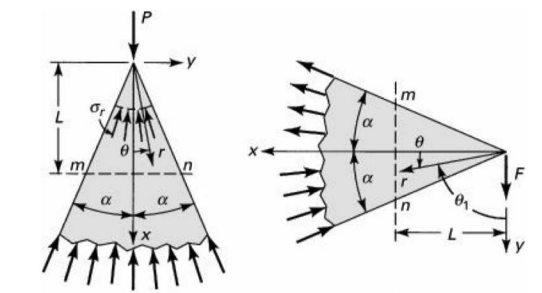
\includegraphics[width=0.3\linewidth]{Questions/Figures/Q3ProblemDiagram.png}
    \caption{Problem diagram for Question 3.}
    \label{fig:Q3ProblemDiagram}
\end{figure}

\subsection{}
The biharmonic equation is
\begin{equation*}
    \nabla^4 \Phi = \frac{\partial^4 \Phi}{\partial x^4} + 2 \frac{\partial^4 \Phi}{\partial x^2 \partial y^2} + \frac{\partial^4 \Phi}{\partial y^4} = 0
\end{equation*}
Substituting $\Phi$ into the biharmonic equation,
\begin{align*}
    \frac{\partial^4 \Phi}{\partial x^4} &= 0 \\
    \frac{\partial^4 \Phi}{\partial y^4} &= 120dy \\
    \frac{\partial^4 \Phi}{\partial x^2 \partial y^2} &= \frac{\partial^2}{\partial x^2} \left(6cy + 20dy^3 + 6ex^2y\right) = 12ey \\
    \implies \nabla^4 \Phi &= 0 + 2(12ey) + 120dy \overset{\text{set}}{=} 0 \\
    \implies e = -5d
\end{align*}
Therefore, $\Phi$ is biharmonic when $\boxed{e = -5d}$.

\subsection{}
The stress function can now be expressed as
\begin{equation*}
    \Phi = ax^2 + bx^2y + cy^3 + dy^5 - 5dx^2y^3 = ax^2 + bx^2y + cy^3 + d(y^5-5x^2y^3)
\end{equation*}
The boundary conditions are
\begin{align*}
    \tau_{xy}|_{y=\pm h} &= 0 \\
    \sigma_y|_{y=h} &= \frac{-pL}{Lt} = -\frac{p}{t} \\
    \sigma_y|_{y=-h} &= 0
\end{align*}
Since there is no axial load,
\begin{equation*}
    \int_{-h}^{h} \sigma_x y dy = 0
\end{equation*}
Finding expressions for $\sigma_x$, $\sigma_y$, and $\tau_{xy}$,
\begin{align*}
    \sigma_x &= \frac{\partial^2 \Phi}{\partial y^2} = 6cy + 20dy^2 - 30dx^2y \\
    \sigma_y &= -\frac{\partial^2 \Phi}{\partial x^2} = 2a + 2by - 10dy^3 \\
    \tau_{xy} &= -\frac{\partial^2 \Phi}{\partial x \partial y} = -2bx + 30dxy^2
\end{align*}
Applying the boundary conditions, first at $\tau_{xy}|_{y=h}$,
\begin{align*}
    \tau_{xy}|_{y=h} &= 0 \\
    \implies -2bx + 30dxh^2 &= 0 \\
    \implies b &= 15dh^2
\end{align*}
second at $\sigma_y|_{y=-h}$,
\begin{align*}
    \sigma_y|_{y=-h} &= 0 \\
    \implies 2a + 2(15dh^2)(-h) - 10d(-h)^3 &= 0 \\
    \implies a &= 10dh^3 
\end{align*}
lastly at $\sigma_y|_{y=h}$,
\begin{align*}
    \sigma_y|_{y=h} &= -\frac{p}{t} \\
    \implies 2(10dh^3) + 2(15dh^2)(h) - 10d(h)^3 &= -\frac{p}{t} \\
    \implies d &= \frac{p}{40h^3 t}
\end{align*}





% \section{}
A displacement field in a body is given by
\begin{align*}
    u = c(x^2 + 10) \\
    v = 2cyz \\
    w = c(-xy+z^2)
\end{align*}

where $c= 10^{-4}$. Determine the state of strain on an element position at (0, 2, 1). 

Calculate all 6 unique entries of the strain tensor:
\begin{align*}
    \epsilon_{x}|_{(0,2,1)} &= \frac{\partial u}{\partial x} = 2cx = 2(10^{-4})(0) = 0 \\ 
    \epsilon_{y}|_{(0,2,1)} &= \frac{\partial v}{\partial y} = 2cz = 2(10^{-4})(1) = 2(10^{-4}) \\
    \epsilon_{z}|_{(0,2,1)} &= \frac{\partial w}{\partial z} = 2cz = 2(10^{-4})(1) = 2(10^{-4}) \\
    \epsilon_{xy}|_{(0,2,1)} &= \frac{1}{2}\left(\frac{\partial u}{\partial y} + \frac{\partial v}{\partial x}\right) = \frac{1}{2}(0 + 0) = 0 \\
    \epsilon_{xz}|_{(0,2,1)} &= \frac{1}{2}\left(\frac{\partial u}{\partial z} + \frac{\partial w}{\partial x}\right) = \frac{1}{2}(0 + -cy) 
    = \frac{1}{2}(0 + -2(10^{-4}) = -10^{-4} \\
    \epsilon_{yz}|_{(0,2,1)} &= \frac{1}{2}\left(\frac{\partial v}{\partial z} + \frac{\partial w}{\partial y}\right) = \frac{1}{2}(2cy + -cx)
    = \frac{1}{2}(2(10^{-4})(2) + 0) = 2(10^{-4})
\end{align*}

Therefore, the strain tensor is
\begin{empheq}[box=\widefbox]{align*}
    % factor out 10^-4
    \epsilon = \begin{bmatrix}
        0 & 0 & -1 \\
        0 & 2 & 2 \\
        -1 & 2 & 2
    \end{bmatrix} \times 10^{-4}
\end{empheq}


% \section{}
The symmetrical frame shown in Fig. \ref{fig:Q5} supports a uniform loading of $p$ per unit length. Assume that each horizontal and vertical
member has the modulus of rigidity $E_1 I_1$ and $E_2 I_2$, respectively. Determine the resultant $R_A$ at the left support, employing
Castigliano's theorem.

\begin{figure}[h]
    \centering
    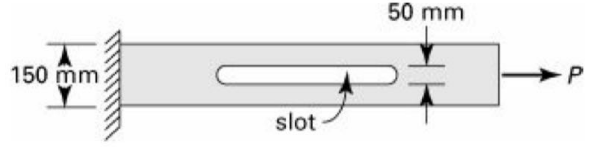
\includegraphics[width=0.5\linewidth]{Questions/Figures/Q5ProblemDiagram.png}
    \caption{Symmetrical frame}
    \label{fig:Q5}
\end{figure}

From A to D, the moment equation is:
\begin{align*}
    M_{AD} &= - R_{Ax} x \\
    \implies \frac{\partial M_{AD}}{\partial R_{Ax}} &= -x
    \implies \frac{\partial M_{AD}}{\partial R_{Ay}} = 0
\end{align*}

From D to F, the moment equation is:
\begin{align*}
    M_{DF} &= M_{AD}|_{x=L_2} + R_{Ay}x - \frac{px^2}{2} \\
    &= -R_{Ax}L_2 + R_{Ay}x - \frac{px^2}{2} \\
    \implies \frac{\partial M_{DF}}{\partial R_{Ax}} &= -L_2 \\
    \implies \frac{\partial M_{DF}}{\partial R_{Ay}} &= x
\end{align*}

From B to E, the moment equation is:
\begin{align*}
    M_{BE} &= 0 \\
    \implies \frac{\partial M_{EB}}{\partial R_{Ax}} &= 0 \\
    \implies \frac{\partial M_{EB}}{\partial R_{Ay}} &= 0
\end{align*}

From C to F, the moment equation is:
\begin{align*}
    M_{CF} &= M_{DF}|_{x=2L_1}  \\ 
    &= -R_{Ax}L_2 + 2R_{Ay}L_1 - 2pL_1^2 \\
    \implies \frac{\partial M_{CF}}{\partial R_{Ax}} &= -L_2 \\
    \implies \frac{\partial M_{CF}}{\partial R_{Ay}} &= 2L_1
\end{align*}

By Castigliano's theorem, the horizontal deflection at A is:
\begin{align*}
    \delta_{A,x} = & \frac{1}{E_1I_1} \left[\int_{0}^{L_2} M_{AD} \left(\frac{\partial M_{AD}}{\partial R_{Ax}}\right) dx
    + \cancel{\int_{0}^{L_2} M_{BE} \left(\frac{\partial M_{BE}}{\partial R_{Ax}}\right) dx}
    + \int_{0}^{L_2} M_{CF} \left(\frac{\partial M_{CF}}{\partial R_{Ax}}\right) dx
    \right] \\
    &+ \frac{1}{E_2I_2} \left[\int_{0}^{2 L_1} M_{DF} \left(\frac{\partial M_{DF}}{\partial R_{Ay}}\right) dx \right] \\
    &= \frac{1}{E_1I_1} \left[\int_{0}^{L_2} R_{Ax} x^2 dx + \int_{0}^{L_2} (-R_{Ax}L_2 + 2R_{Ay}L_1 - 2pL_1^2)(-L_2) dx \right] \\
    &+ \frac{1}{E_2I_2} \left[\int_{0}^{2 L_1} (-R_{Ax}L_2 + R_{Ay}x - \frac{px^2}{2})x dx \right] \\
    &= \frac{1}{E_1I_1} \left[\frac{L_2^3R_{Ax}}{3} + L_2^2(2pL_1^2 - 2R_{Ay}L_1 + L_2R_{Ax}) \right]
    - \frac{1}{E_2I_2} \left[\frac{2pL_1^4}{3} - \frac{2R_{Ay}L_1^3}{3} + \frac{L_2R_{Ax}L_1^2}{2} \right] \\
\end{align*}

Since the pin at A cannot carry deflection, $\delta_{A,x} = 0$. Therefore,
\begin{align*}
    \delta_{A,x} \overset{\text{set}}{=} 0 \\
    \implies R_{Ax} &= -\frac{\frac{L_{2}^2 (2 L_{1}^2 - 2L_1 R_{Ay})}{E_1 I_1} + \frac{\frac{8L_{1}^3 R_{Ay}}{3} - \frac{2L_{1}^4 p}{3}}{E_2 I_2}}
    {\frac{4L_{2}^3}{3 E_1 I_1} - \frac{2L_{1}^2 L_{2}}{E_2 I_2}} 
\end{align*}
By Castigliano's theorem, the vertical deflection at A is:
\begin{align*}
    \delta_{A, y} = &\frac{1}{E_1I_1} \left[\cancel{\int_{0}^{L_2} M_{AD} \left(\frac{\partial M_{AD}}{\partial R_{Ay}}\right) dx}
    + \cancel{\int_{0}^{L_2} M_{BE} \left(\frac{\partial M_{BE}}{\partial R_{Ay}}\right) dx}
    + \int_{0}^{L_2} M_{CF} \left(\frac{\partial M_{CF}}{\partial R_{Ay}}\right) dx
    \right] \\
    &+ \frac{1}{E_2I_2} \left[\int_{0}^{2 L_1} M_{DF} \left(\frac{\partial M_{DF}}{\partial R_{Ay}}\right) dx \right] \\
    &= \frac{1}{E_1I_1} \left[\int_{0}^{L_2} (-R_{Ax}L_2 + 2R_{Ay}L_1 - 2pL_1^2)(2L_1) dx \right]
    + \frac{1}{E_2I_2} \left[\int_{0}^{2 L_1} (-R_{Ax}L_2 + R_{Ay}x - \frac{px^2}{2})(x) dx \right] 
\end{align*}
Too much algebra, by Matlab Symbolic Toolbox:
\begin{verbatim}
ans = 

struct with fields:

Rax: (3*E1*I1*L1^2*p*(2*L1^2 + L2*L1))/(L2*(6*E1*I1*L1^2 + E1*I1*L1*L2 - 3*E2*I2*L2^2))
Ray: (3*L1*p*(3*E1*I1*L1^2 + E1*I1*L1*L2 - E2*I2*L2^2))/...
(6*E1*I1*L1^2 + E1*I1*L1*L2 - 3*E2*I2*L2^2)
\end{verbatim}
The script was used to aid in this solution:
\begin{verbatim}
clc; clear; close all;
syms x L1 L2 p Rax Ray E1 I1 E2 I2
delta_Ax = (1/(E1*I1)) * (int(Rax*x^2, x, 0, L2) + int((-Rax*L2 + 2*Ray*L1 - 2*p*L1^2)*(-L2)...
    , x, 0, L2)) + (1/(E2*I2)) * (int((-Rax*L2 + Ray*x - (p*x^2)/2)*x, x, 0, 2*L1))

delta_Ay = (1/(E1*I1)) * (int((-Rax*L2 + 2*Ray*L1 - 2*p*L1^2)*(2*L1), x, 0, L2)) ...
    + (1/(E2*I2)) * (int((-Rax*L2 + Ray*x - (p*x^2)/2)*(x), x, 0, 2*L1))

eqn1 = delta_Ax == 0;
eqn2 = delta_Ay == 0;
solve(eqn1, Rax)
solve([eqn1, eqn2], [Rax, Ray])
\end{verbatim}
% \section{}
Find the normal strain in the members $\overline{AB}$ and $\overline{BC}$ of the pin-connected plane structure shown in
Fig.(\ref{fig:q6problem}) if point B is moved leftward 2.5 mm. Assume that axial deformation is uniform throughout
the length of each member.


\begin{figure}[h]
    \centering
    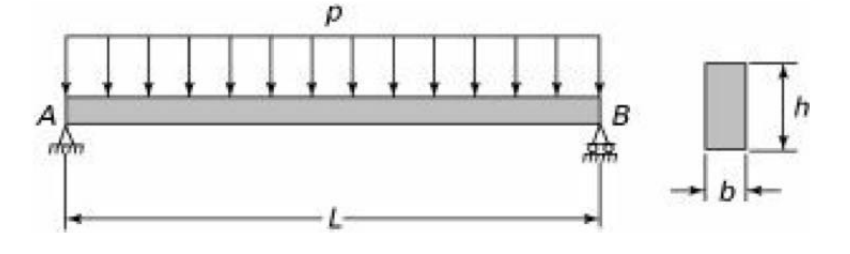
\includegraphics[width=0.3\linewidth]{Questions/Figures/Q6ProblemDiagram.png}
    \caption{Pin connected plane structure}
    \label{fig:q6problem}
\end{figure}

Convert the displacement of point B with respect to point A to a strain:
\begin{align*}
    \epsilon_{AB} &= \frac{\Delta L}{L} = \frac{-2.5 e-3}{1.8} = \boxed{\qty{-1.39e-3}{}}
\end{align*}

Find the displacement of point B with respect to point C:
\begin{align*}
    l_{BC, f} &= \sqrt{2.4^2 + (1.8 - 2.5\times 10^{-3})^2} = \qty{2.9985}{\meter} \\
    \Delta l_{BC} &= l_{BC, f} - l_{BC, i} = 2.9985 - 3.0 = \qty{-1.50 e-3}{\meter}
\end{align*}

Convert the displacement of point B with respect to point C to a strain:
\begin{align*}
    \epsilon_{BC} &= \frac{\Delta L}{L} = \frac{-1.5 e-3}{3.0} = \boxed{\qty{-5.00e-4}{}}
\end{align*}

  

% \newpage
% %\bibliographystyle{IEEEtran}
% %\bibliography{citations.bib}
% %\bibliography{}

% \newpage
% \appendix
% \sectionfont{\large}
\section{Appendix: Matplotlib Python Code to Render Graphs}
This is just some random code.
\begin{lstlisting}[language=Python]
if transactions: Transaction.create_transactions() # if transactions = "true"
node.generate_emptyState() # empty state for all nodes
S.initial_events() # initiate initial events to start with

while not queue.isEmpty() and clock <= targetTime:
    next_e = queue.get_next_event()
    clock = next_e.time # move clock to the time of the event
    Event.execute_event(next_e)
    Queue.remove_event(next_e)

print results
\end{lstlisting}

\end{document}